\chapter{Project Management}
\section{Agile Development Methodology}
Teams use the agile development methodology to minimize risk (such as bugs, cost overruns, and changing requirements) when adding new functionality. In all agile methods, teams develop the software in iterations that contain mini-increments of the new functionality. There are many different forms of the agile development method, including scrum, crystal, extreme programming (XP), and feature-driven development (FDD).

\begin{figure}[H]
    \centering
    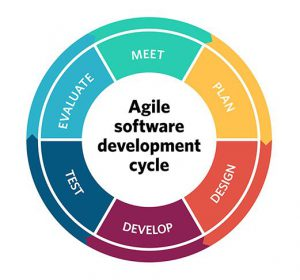
\includegraphics[scale = 0.9]{agile.jpg}
    \caption{Agile Development Methodology}
    \label{fig:Agile Development Methodology}
\end{figure}

\section{Trello}
We are going to use Trello's default agile board for task management. 
\begin{figure}[H]
    \centering
    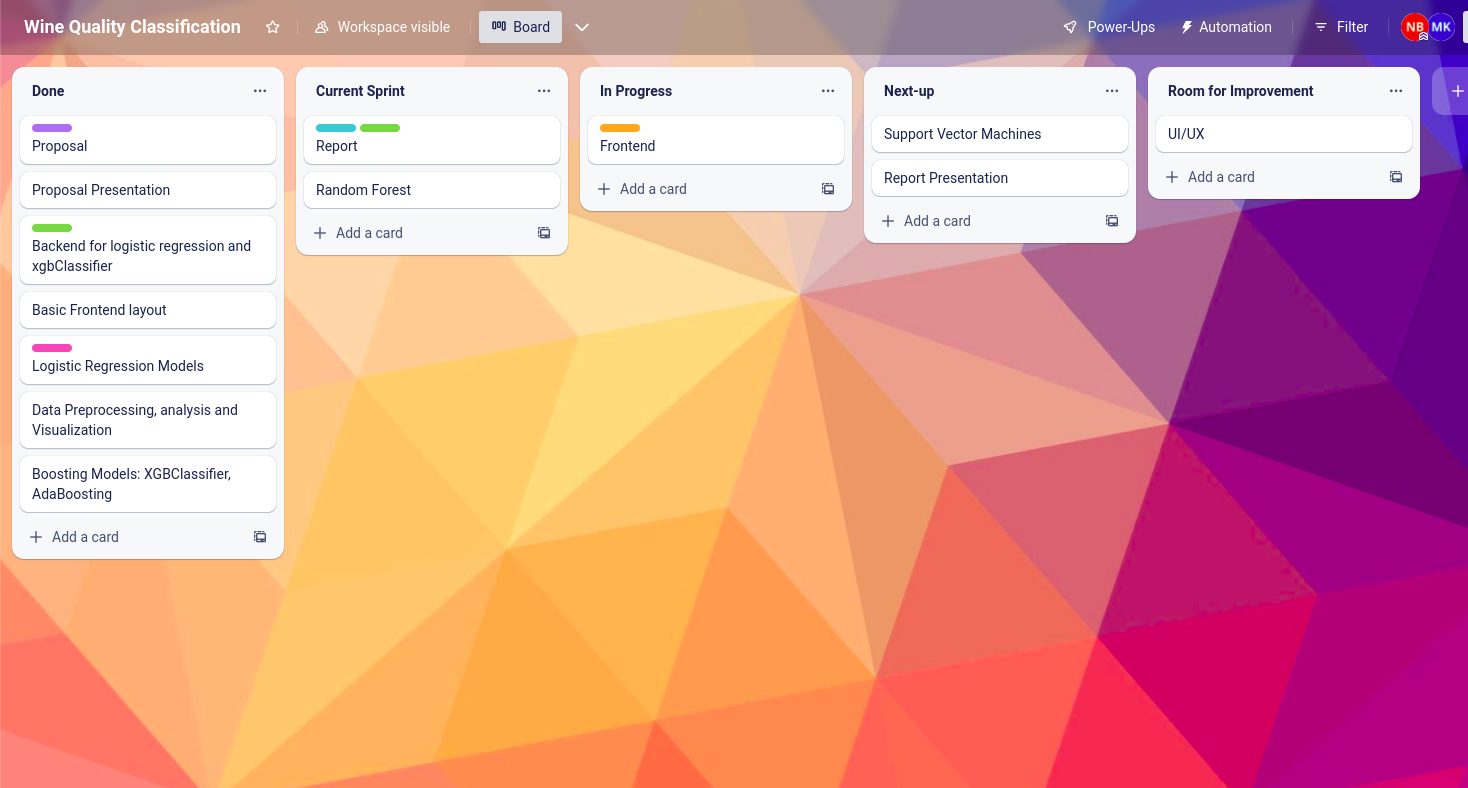
\includegraphics[scale = 0.33]{trello.png}
    \caption{Trello}
    \label{fig:Trello}
\end{figure}

\section{Discord}
We are going to use Discord server for effective communication and team meetings.

\begin{figure}[H]
    \centering
    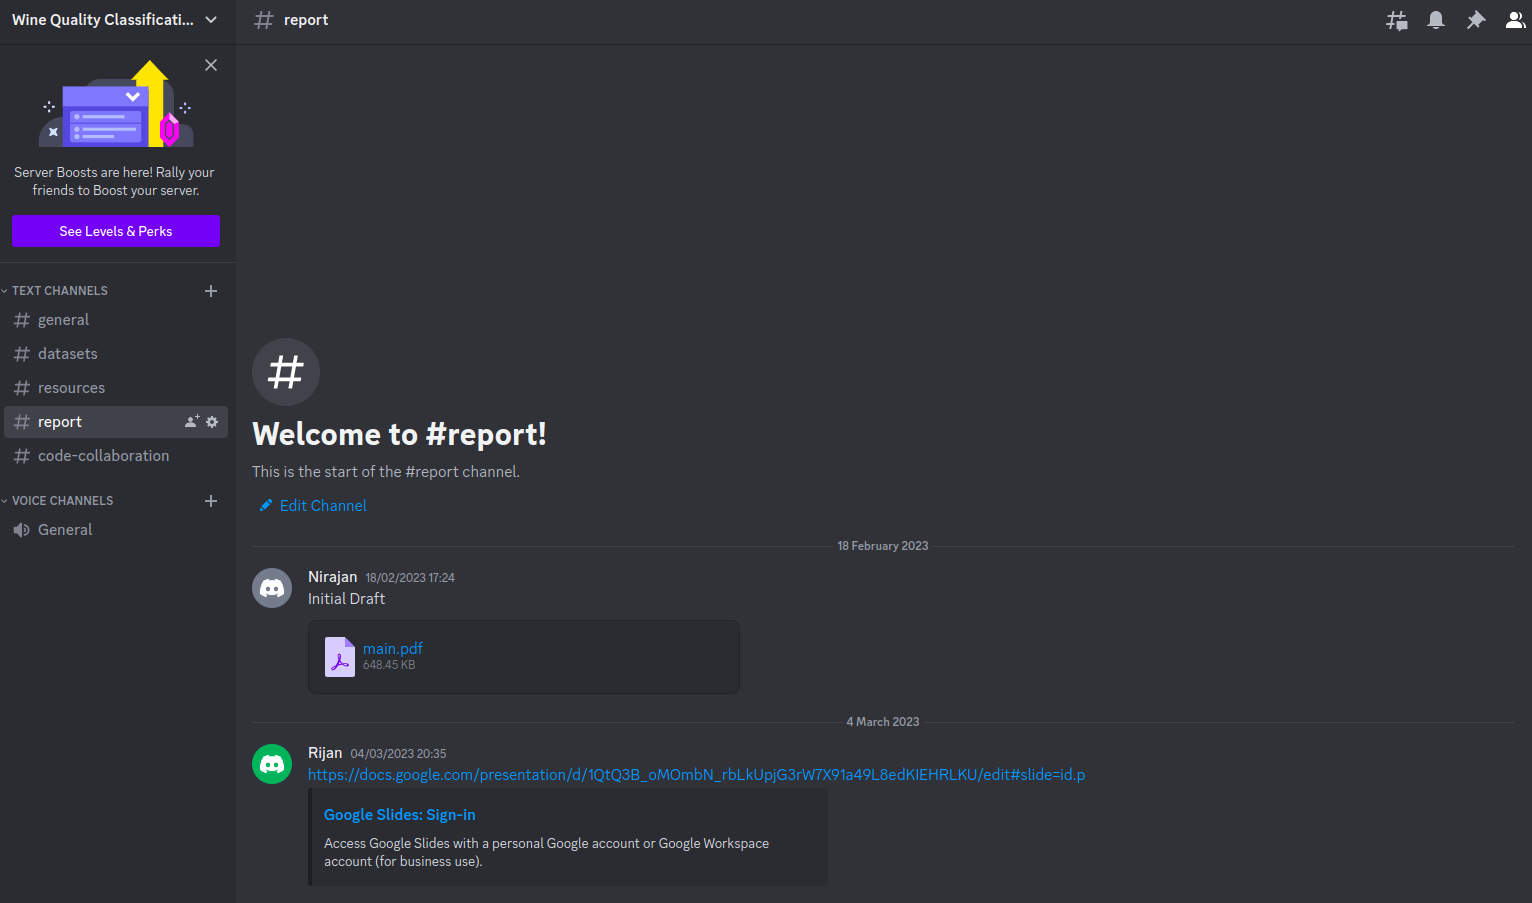
\includegraphics[scale = 0.26]{discord.png}
    \caption{Discord}
    \label{fig:Discord}
\end{figure}

\section{Tensorboard}
Tensorboard will be used for experiment tracking.
\begin{figure}[H]
    \centering
    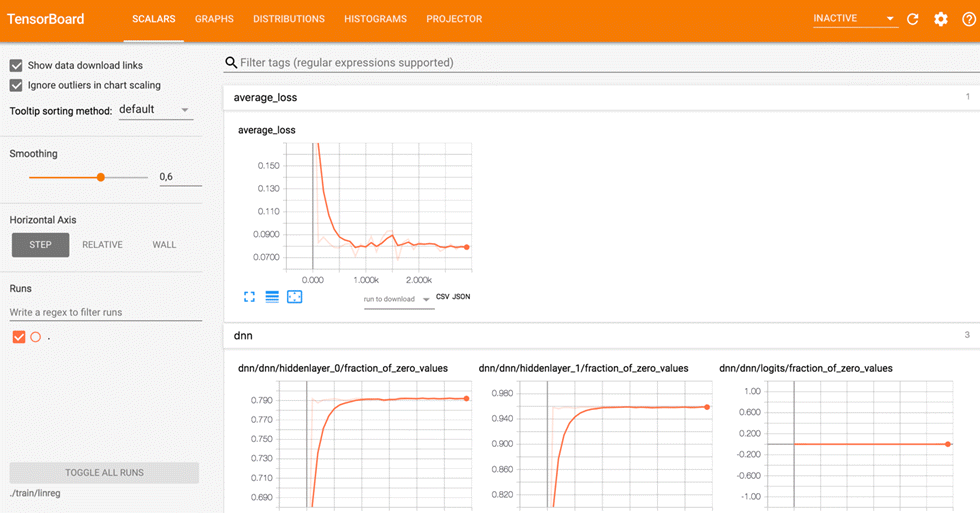
\includegraphics[scale = 0.45]{tensorboard.png}
    \caption{Tensorboard}
    \label{fig:Tensorboard}
\end{figure}

